\documentclass[12pt,a4paper]{article}

\usepackage{lmodern}
\usepackage[T1]{fontenc}
\usepackage[utf8]{inputenc}
\usepackage[italian]{babel}

\usepackage{hyperref}
\usepackage{graphicx}
\graphicspath{{img/}}
\usepackage{float}

\usepackage{titlesec}

\usepackage[a4paper]{geometry}

\usepackage{fancyhdr}
\fancyhf{} % clear all header and footers
\renewcommand{\headrulewidth}{0pt} % remove the header rule
\rfoot{\thepage}

% Turn on the style
 \pagestyle{fancy}

\setcounter{secnumdepth}{4}

\titleformat{\paragraph}
{\normalfont\normalsize\bfseries}{\theparagraph}{1em}{}
\titlespacing*{\paragraph}
{0pt}{3.25ex plus 1ex minus .2ex}{1.5ex plus .2ex}

\begin{document}
\begin{titlepage}
	\centering
	\vspace*{1cm}
	{\scshape\LARGE \textbf{EmpireCon} \par}
	\vspace{0.5cm}
	{\Large \textbf{\textit{Relazione sul progetto per il corso di Tecnologie Web}}\par}
	\vspace{3cm}
	{\Large Andrea Cardin, 1030310\par}
	{\Large Andrea Nalesso, 1026100\par}
	{\Large Ismaele Gobbo, 1028902\par}
	\vspace{6cm}
	{\normalsize \textbf{Indirizzo del sito:} \url{http://tecnologie-web.studenti.math.unipd.it/tecweb/~acardin/}\par}
	{\normalsize \textbf{Utente amministratore:} admin\par}
	{\normalsize \textbf{Password amministratore:} password\par}
	{\normalsize \textbf{Utente comune:} user\par}
	{\normalsize \textbf{Password utente comune:} password\par}
	{\normalsize \textbf{Referente del gruppo:} darktal91@gmail.com (Andrea Cardin)\par}
	\vspace*{\fill}
\end{titlepage}

\tableofcontents
\newpage

% Come inserire una sezione
% \section{Nome sezione}
% \input{sections/nome file latex della sezione senza .tex}
% \newpage
% Esempio:
% \section{Introduzione}
% placeholder
% \newpage

\section{Introduzione}
placeholder

\section{Progettazione}
\subsection{Struttura del sito}
Ogni pagina del sito è formata dai seguenti elementi:
\begin{itemize}
	\item Header;
	\item breadcrumb;
	\item box che permette il login o mostra l'account con cui si è autenticati;
	\item menù;
	\item contenuto della pagina;
	\item footer.
\end{itemize}

\subsubsection{Mappa del sito}
\begin{figure}[H]
	\centering
	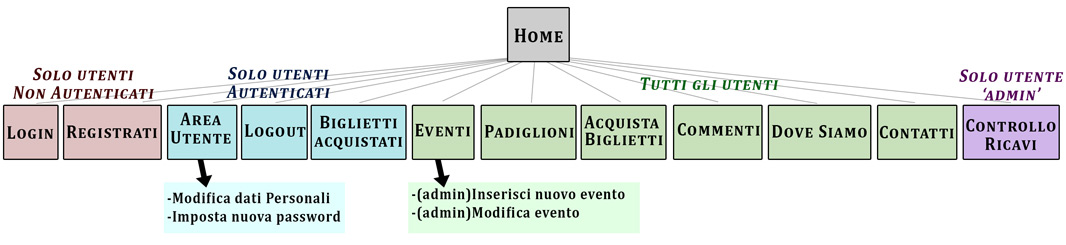
\includegraphics[width=16cm]{mappa-sito-small}
	\caption{Mappa del sito.}
\end{figure}
Oltre alla home page, che è concettualmente la radice del sito ed è ovviamente accessibile a tutti gli utenti, le varie pagine sono concettualmente suddivise nelle seguenti aree basate sull'attore che le andrà ad utilizzare:
\begin{itemize}
	\item Per soli utenti non autenticati;
	\item per soli utenti autenticati;
	\item per tutti gli utenti;
	\item per il solo utente amministratore.
\end{itemize}

\paragraph{Home page}
È, concettualmente, la radice del sito, nonché la pagina in cui l'utente si dovrebbe ritrovare quando si collega al sito. Contiene un paragrafo introduttivo di benvenuto e presentazione, seguito dalle news riguardante l'evento.

\paragraph{Per soli utenti non autenticati}
Quest'area contiene le pagine destinate agli utenti non autenticati, permettendo loro di interagire con le funzioni di autenticazione e registrazione al sito.
Pagine che ne fanno parte:
\begin{itemize}
	\item Login;
	\item Registrazione.
\end{itemize}

\paragraph{Per soli utenti autenticati}
Quest'area contiene le pagine che possono essere visitate o accedute solo dagli utenti che hanno eseguito l'autenticazione al sito. Le pagine di questa area permettono di interagire con gli aspetti relativi alla gestione del proprio account, come ad esempio la modifica dei dati personali o della password, la possibilità di effettuare il logout e, infine, un elenco dei biglietti acquistati da quell'account. L'accesso ad una di queste pagine da parte di un utente non autenticato produce un errore oppure, nel caso di area utente e logout, un reindirizzamento. Inoltre, ad un utente non autenticato non sono mai mostrati collegamenti a queste pagine.
Pagine che ne fanno parte:
\begin{itemize}
	\item Area Utente;
	\item Logout;
	\item Biglietti Acquistati.
\end{itemize}

\paragraph{Per tutti gli utenti}
Queste pagine sono accessibili a tutti gli utenti, a prescindere dal loro stato di autenticazione, tramite il menù.
Contengono i contenuti veri e propri del sito, con informazioni sulla fiera, l'acquisto dei biglietti e la possibilità di lasciare dei commenti.
Pagine che ne fanno parte:
\begin{itemize}
	\item Eventi:
		Presenta la lista di tutti gli eventi che si terranno nel corso della fiera. Per ogni evento vengono offerte informazioni utili quali la data, l'ora di inizio, l'ora di fine, il padiglione in cui si svolgeranno ed una descrizione.
		L'utente amministratore ha la possibilità di svolgere alcune funzioni aggiuntive: l'inserimento di un nuovo evento e la modifica o cancellazione di un evento già inserito.
	\item Padiglioni:
		Mostra l'elenco dei padiglioni presenti nella fiera suddivisi per settori. Inoltre mostra anche una mappa con la posizione di ogni padiglione. Il contenuto è uguale per tutte le categorie di utenti.
	\item Acquista biglietti:
		Elenca a tutti i tipi di utenti le varie tipologie di biglietti disponibili ed il loro prezzo. Ad un utente autenticato offre anche la possibilità di procedere all'acquisto di uno o più biglietti.
	\item Commenti:
		Rappresenta il "libro ospiti" del sito. Gli utenti di tutte le categorie possono leggere i commenti. Un utente autenticato ha a disposizione la funzione di eliminazione per i commenti da lui inviati, mentre l'utente amministratore può eliminare qualsiasi commento.
	\item Dove siamo:
		Offre indicazioni per raggiungere il luogo della fiera. Il contenuto è uguale per tutte le categorie di utenti.
	\item Contatti:
		Contiene informazioni su come contattare gli organizzatori della fiera. Il contenuto è uguale per tutte le categorie di utenti.
\end{itemize}

\paragraph{Per il solo utente amministratore}
A questa categoria appartiene una sola pagina: Controllo ricavi.
Questa pagina è destinata all'utente amministratore e presenta in forma tabellare il resoconto sui biglietti venduti e sui guadagni.

\subsection{Layout}
\textbf{TODO}

\subsection{scelte progettuali}
\textbf{TODO}

	

\section{Realizzazione}
\subsection{Perl}
Per la componente dinamica e di back-end del sito è stato utilizzato il linguaggio Perl come richiesto dalle specifiche del progetto. La versione utilizzata è quella installata nel server tecweb dell'Università. \newline
Le librerie principali utilizzate, dopo una iniziale valutazione tra quelle disponibili, sono state:
\begin{itemize}
	\item \textbf{CGI:} Per la gestione delle connessioni, il passaggio dei parametri HTTP tra le pagine e la gestione delle sessioni;
	\item \textbf{LibXML:} Per la gestione e manipolazione dei file XML;
	\item \textbf{HTML::Template:} Per la costruzione e presentazione dei contenuti. 
\end{itemize}
Tutte le pagine del sito sono dinamiche e realizzate in Perl per poter gestire le sessioni e le operazioni degli utenti.
Ogni pagina è realizzata in maniera modulare tramite template innestati. L'elemento principale è il template \textit{Page} che contiene il menù e il breadcrumb del sito, nonché richiama l'inclusione di altri template: \textit{Header}, che contiene il blocco \textit{head} della pagina, ed il \textit{Footer}. Oltre ai template sopraccitati, che sono presenti in ogni pagina e adattati tramite variabili dinamiche, il template Page richiede l'inclusione del contenuto vero e proprio della pagina, che è stato realizzato sotto forma di un template specifico per ogni pagina del sito. La dinamicità dei contenuti è ottenuta tramite l'interazione (sotto forma di variabili) tra il template del contenuto e la corrispondente pagina cgi.
La libreria LibXML è stata scelta perché è risultata essere la più completa e di più semplice utilizzo.

\subsection{XML}
Il progetto include quattro file XML utilizzati per salvare in modo persistente i dati. Per ogni file XML è stato realizzato un XMLSchema che ne definisce la struttura. Gli schemi sono stati realizzati utilizzando il modello \textit{Tende alla Veneziana}. Utilizzando il tool \textit{xmllint} gli schemi sono stati validati contro lo schema che definisce gli XMLSchema fornito dal W3C, mentre i file XML sono stati validati contro i rispettivi schemi da noi scritti. \newline
I file XML realizzati sono:
\begin{itemize}
	\item \textbf{utenti:} contiene tutti i dati degli utenti che si registrano al sito, compresi username e password necessari per l'autenticazione. La password viene cifrata con una funzione di hash prima di essere salvata;
	\item \textbf{commenti:} contiene tutti i commenti inviati dagli utenti;
	\item \textbf{eventi:} contiene tutti gli eventi che avranno luogo durante la fiera;
	\item \textbf{biglietti:} contiene la lista di tutti i biglietti acquistati.
\end{itemize}

\section{Accessibilità e test}
Per garantire che il sito sia accessibile al maggior numero di utenti e dispositivi è stato realizzato tenendo in considerazione le linee guida del WCAG. \newline

\subsection{Immagini}
L'uso di immagini come contenuto è stato estremamente limitato. In ogni caso per ognuna delle immagini di contenuto utilizzate è stato fornito un attributo \textit{alt} non vuoto contenente una descrizione dell'immagine. Il corretto funzionamento degli attributi \textit{alt} è stato verificato usando l'estensione per chrome \textit{Image Alt Text Viewer}.

Per la mappa dei padiglioni, presente nella pagina \textit{Padiglioni}, non è stata fornita una descrizione dettagliata perché l'immagine non offre particolari informazioni aggiuntive rispetto all'elenco testuale presente di fianco, è solo un supporto visivo aggiuntivo per orientarsi. Inoltre, una descrizione dettagliata della mappa avrebbe richiesto l'utilizzo dell'attributo \textit{longdesc}, il quale però è scarsamente supportato dai browser.

\subsection{Colori e contrasto}
La scelta dei colori per il sito è stata fatta tenendo in considerazione la presenza di diffusi problemi visivi tra la popolazione, e quindi probabilmente anche tra gli utenti. I colori sono stati scelti in modo da garantire sempre un contrasto elevato tra le varie parti. Per verificare il contrasto tra i colori del testo e i quelli dello sfondo nella parte di contenuto delle pagine è stato usato il sito \url{https://snook.ca/technical/colour_contrast/colour.html}, che ha dato esito positivo.

Inoltre, utilizzando l'estensione \textit{Spectrum} per il browser chorome è stato testato il comportamento della grafica del sito in caso di vari tipi di daltonismo. I risultati sono stati buoni in alcuni casi e accettabili in altri. Un unico elemento del sito è risultato problematico per un tipo di daltonismo: il link alla home nella breadcrumb. Purtroppo, a causa di mancanza di tempo, non è stato possibile risolvere questo problema, perché il colore di quel link è conforme al colore di tutti i link di contenuto del sito, e cambiare la colorazione della barra che contiene la bradcrumb avrebbe richiesto di cambiare anche quasi tutti gli altri colori della grafica. Tuttavia questo problema non è particolarmente grave: l'informazione che si perde non è di vitale importanza considerando la struttura molto semplice del sito e la presenza di un link alla home page nel menù sottostante.

\subsection{Markup e fogli di stile}
Per garantire la massima compatibilità possibile con i vari dispositivi il sito è stato realizzato rispettando lo standard XHTML Strict e le linee guida W3C. Tutte le pagine sono state validate utilizzando il validatore del W3C (\url{https://validator.w3.org}). \newline
I fogli di stile sono stati realizzati utilizzando CSS puri e validati usando il sito \url{https://jigsaw.w3.org/css-validator/}.

\subsection{Lingua}
La lingua principale del sito è l'italiano. Nei casi in cui sono stati inseriti termini non appartenenti alla lingua italiana essi sono stati rinchiusi in un marcatore che ne dichiarasse la lingua di appartenenza, ad esempio <span xml:lang="en">...</span>. Questo accorgimento serve per permettere agli screen reader di leggere tali termini utilizzando la corretta pronuncia.

\subsection{Tabelle}
Nel sito è stata utilizzata una sola tabella nella pagina \textit{Controllo Ricavi}, destinata al solo utente amministratore. Per renderla accessibile è stato specificato attentamente l’attributo \textit{"summary"} ed inserito l’attributo \textit{"scope=col"} negli header. \newline
Per quanto riguarda l'attributo "summary", è stato preso come modello l'esempio realizzato da Michele Diodati nel suo libro \textit{Accessibilità - Guida Completa}, al capitolo 8 (Punto di controllo 5.5, priorità 3). \newline
È stata inoltre verificata la corretta visualizzazione della tabella provando su più browser e dispositivi.

\subsection{Compatibilità e portabilità}
Il sito è stato progettato e realizzato con l'obiettivo di essere usabile dal maggior numero di utenti possibile, anche se non provvisti di browser di ultima generazione. 
Sono stati effettuati test con i seguenti browser desktop:
\begin{itemize}
	\item Internet Explorer 8;
	\item Internet Explorer 11;
	\item Edge versione 25;
	\item Chrome versione 52;
	\item Mozilla Firefox versione 41.
\end{itemize}
E sui seguenti browser mobile:
\begin{itemize}
	\item Silk versione 52 (browser Kindle Fire);
	\item Chrome per Android versione 52.
\end{itemize}
Inoltre, è stata testata la navigazione utilizzando il browser testuale Lynx.

\subsection{Dinamicità}
Per evitare di creare problemi o disturbo agli utenti con testi o immagini in movimento tutti i contenuti del sito sono statici.

\subsection{Indipendenza dal dispositivo}
Il sito è stato progettato e realizzato con l'obiettivo di essere agevolmente navigabile sia tramite computer che tramite dispositivi mobile (smartphone e tablet).
I membri del gruppo hanno testato il sito utilizzando tutti i dispositivi in nostro possesso ed è risultato visitabile in tutti i casi. \newline
In ogni caso la struttura di HTML e CSS è stata realizzata seguendo le linee guida di WCAG per l'accessibilità, quindi è ragionevole supporre che il sito sia visitabile con qualsiasi dispositivo.

\subsection{Contesto e aiuto per l'orientamento}
Anche se la struttura del sito è molto semplice, in ogni pagina è presente una \textit{breadcrumb} che permette all'utente di sapere sempre in che posizione si trova all'interno del sito. Inoltre, il titolo di ogni pagina identifica chiaramente la stessa. \newline
All'interno del contenuto sono stati inseriti dei link, dove necessario, per permettere all'utente di spostarsi agevolmente all'interno del sito. Ad esempio nelle pagine in cui è richiesta l'autenticazione per svolgere alcune operazioni è presente, accanto alla spiegazione della necessità dell'autenticazione, un collegamento alla pagina di login.

\subsection{Link}
Per quanto riguarda il testo dei link, si è cercato di renderlo il più chiaro possibile anche al di fuori del suo contesto

Per la colorazione dei link all'interno dei contenuti del sito è stato scelto di utilizzare dei colori diversi da quelli standard per ottenere una maggior integrazione con il resto della grafica. I link visitati cambiano colore.

I link del menù, invece, non cambiano colore quando visitati. Questa scelta, benché non ottimale e non in linea con le raccomandazioni, non dovrebbe comportare disorientamento nell'utente durante la navigazione perché il numero di pagine è estremamente ridotto, la struttura del sito è molto semplice e inoltre è presente una breadcrumb.

\subsection{Screen reader}
Nell'analisi delle caratteristiche degli utenti a cui il sito è indirizzato non si è ritenuta significativa la fascia di utenti non vedenti, in quanto la saga di Star Wars deve buona parte del suo successo all'impatto visivo ed agli effetti speciali. \newline
Tuttavia, il sito è risultato perfettamente usabile tramite browser testuale, ed è stato realizzato seguendo le linee guida di accessibilità, quindi ci si aspetta che risulti navigabile anche utilizzando uno screen reader.




\section{Suddivisione dei ruoli}
\begin{table}[H]
	\centering
	\caption{Suddivisione dei ruoli}
	\begin{tabular}{|l|p{0.55\textwidth}|}
		\hline
		\multicolumn{1}{|c|}{\textbf{Persona}} & \multicolumn{1}{c|}{\textbf{Ruoli}}                   \\ \hline
\multicolumn{1}{|l|}{\rule{0pt}{4ex} Andrea Cardin}  & \multicolumn{1}{p{0.55\textwidth}|}{ \begin{itemize}
			\setlength{\itemsep}{0pt}
			\setlength{\parskip}{0pt}
			\setlength{\parsep}{0pt} 
			\item Configurazione ambiente di lavoro;
			\item progettazione struttura del sito;
			\item creazione pagine dinamiche in Perl;
			\item creazione template e struttura XHTML;
			\item contenuti pagine XHTML;
			\item stesura XMLSchema;
			\item popolamento banca dati XML;
			\item test di usabilità;
			\item validazione;
			\item stesura e verifica della relazione.
		\end{itemize} } \\ \hline
\multicolumn{1}{|l|}{\rule{0pt}{4ex} Andrea Nalesso} & \multicolumn{1}{p{0.55\textwidth}|}{
	\begin{itemize}
		\setlength{\itemsep}{0pt}
		\setlength{\parskip}{0pt}
		\setlength{\parsep}{0pt} 
		\item progettazione struttura del sito;
		\item creazione pagine dinamiche in Perl;
		\item creazione template e struttura XHTML;
		\item contenuti pagine XHTML;
		\item stesura XMLSchema;
		\item popolamento banca dati XML;
		\item test di accessibilità;
		\item test di usabilità;
		\item validazione;
		\item stesura e verifica della relazione.
	\end{itemize}} \\ \hline
	\multicolumn{1}{|l|}{\rule{0pt}{4ex} Ismaele Gobbo}  & \multicolumn{1}{p{0.55\textwidth}|}{\begin{itemize}
			\setlength{\itemsep}{0pt}
			\setlength{\parskip}{0pt}
			\setlength{\parsep}{0pt} 
			\item progettazione struttura del sito;
			\item contenuti pagine XHTML;
			\item progettazione interfaccia;
			\item CSS desktop;
			\item CSS mobile;
			\item CSS print;
			\item test di accessibilità;
			\item test di usabilità;
			\item validazione;
			\item stesura e verifica della relazione.
		\end{itemize}} \\ \hline
\end{tabular}
\end{table}
\end{document}
